%%%%%%%%%%%%%%%%%%%%%%%%%%%%%%%%%%%%%%%%%%%%%%%%%%%%%%%%%%%%%%%%%%%%%%%%%%%%
\documentclass[dvipdfmx,a4j]{jarticle}

\usepackage{jsaisig}
\usepackage{amsmath,amssymb}
\usepackage{graphicx}
\usepackage{bm}
\usepackage{booktabs}
\usepackage{multirow}

\setlength{\textfloatsep}{10pt}
\setlength{\abovecaptionskip}{3pt}
\setlength{\belowcaptionskip}{0pt}
\renewcommand{\baselinestretch}{0.95}

\newcommand{\argmax}{\mathop{\rm argmax}\limits}

%%%%%%%%%%%%%%%%%%%%%%%%%%%%%%%%%%%%%%%%%%%%%%%%%%%%%%%%%%%%%%%%%%%%%%%%%%%

\begin{document}

\title{回答履歴を考慮した強化学習に基づく適応型テスト}
\etitle{Adaptive Testing Based on Reinforcement Learning Considering Response History}

\author{柴沼 厳 \ \ 宇都 雅輝}

\affiliation{%
	電気通信大学\\
	The University of Electro-Communications}

\abstract{
コンピュータ適応型テスト（Computerized Adaptive Testing: CAT）における項目選択は，受検者の特性値を効率的に推定するための中核的な過程である．近年，深層強化学習を用いた項目選択戦略として，Deep Q-Network（DQN）に基づく手法が提案され，従来の情報量基準手法を上回る推定精度が報告されている．しかし，DQN に基づく手法では，状態として現在推定されている特性値のみを用いるため，受検者のこれまでの回答パターンに含まれる情報を十分に活用できていない．本研究では，IRT に基づく CAT を部分観測マルコフ決定過程（POMDP）として再定式化し，受検者の回答履歴を状態として利用する Deep Recurrent Q-Network（DRQN）に基づく項目選択戦略を提案する．3パラメータロジスティックモデル（3PLM）に基づくシミュレーション実験の結果，40問選択時点において，提案手法（DRQN）は RMSE = 0.200 を達成し，MFI（RMSE = 0.342）および DQN（RMSE = 0.254）を上回る推定精度を示した．
}

\maketitle
\thispagestyle{empty}

\section{はじめに}

コンピュータ適応型テスト（CAT）は，スマート・テスティングにおいて広く用いられる手法であり，心理・教育測定における主要な研究テーマでもある~\cite{zhang2016}．紙筆式テストのような非適応型の形式と比べ，CAT はより少ない項目数で受検者の真の特性値をより正確に推定できる．これは，受検者の反応に加え，内容バランスや露出制御といった制約も考慮しつつ，統計的に最も情報量の高い項目群を提示することで達成される~\cite{weiss1982,wainer2000,frey2023}．

効率的な測定を実現する中核過程である項目選択は，CAT における重要な研究焦点である．従来の項目選択戦略の多くは，項目反応理論（Item Response Theory: IRT）の枠組みの下で提案されている~\cite{vanderlinden2016}．最も広く使われる方法は，フィッシャー情報量を最大化する項目を選ぶ最大フィッシャー情報量法（Maximum Fisher Information: MFI）である~\cite{lord1980}．MFI は推定された特性値の漸近分散の逆数を最大化するという明快な原理に基づくが，推定特性値が真の特性値から大きく乖離している場合には，最も情報量の高い項目を選択できないという問題がある~\cite{chang1996}．この問題に対処するため，尤度で重み付けしたフィッシャー情報量（FIWL）~\cite{veerkamp1997} や，尤度重み付き Kullback-Leibler 情報量（KLP）~\cite{chang1996} などの代替戦略が提案されてきた．

しかし，これらの情報量基準に基づく項目選択戦略には，根本的な限界がある．第一に，従来の戦略の多くは全体最適ではなく局所最適な選択を行う．ほとんどの戦略は次の1項目に関する情報のみを考慮するため，さらに数項目先まで見越して得られる潜在的情報を取り込むことが難しい．第二に，従来の戦略は他の受検者の受検記録から情報を掘り起こして効率を高めることができない．過去の受検記録から学習できる柔軟な枠組みに基づく選択戦略であれば，特性値推定の変化の軌跡や，将来得られるテスト情報を予測できる可能性がある．

これらの限界に対処する有望なアプローチが強化学習（Reinforcement Learning: RL）である~\cite{sutton2018}．深層学習と組み合わせた深層強化学習は，さまざまな先端領域で従来手法や人間の能力を上回る成果を示してきた~\cite{silver2016,silver2017}．近年，RL は適応学習システムにおける教材推薦など，教育測定における長期的かつ適応的な目的をもつ問題の解決に適合し強力であることが示されている~\cite{chen2018,han2020,li2021,li2023,tan2020,tang2019}．CAT においても，分類型 CAT に対する DRL ベースの選択戦略~\cite{nurakhmetov2019} や，二段階最適化に基づく枠組み~\cite{ghosh2021}，形成的評価への適用~\cite{shin2022} など，RL の導入が試みられている．

しかし，CAT への RL 導入に関する既存研究にはいくつかのギャップが残る．第一に，3PLM のような最も一般的な IRT モデルに基づく CAT について，RL 枠組みの定義や選択戦略の提案がなされていない．第二に，既存研究で多く用いられるアクター・クリティック法は大量の学習データを要する．第三に，RL ベースの戦略が長期的情報を考慮することで測定精度を改善できるかどうか，従来の IRT ベース戦略との体系的な比較が不足している．

これらのギャップに対し，Wang ら~\cite{wang2024} は CAT の項目選択問題をマルコフ決定過程（MDP）として定式化し，DQN を用いて Q 関数を近似する手法を提案した．この手法は，現在の項目だけでなく将来のテスト全体で得られる情報量の期待値を最大化するように項目を選択するため，局所最適に陥りやすい従来手法の課題を緩和する．シミュレーションおよび実データを用いた実験において，DQN は MFI をはじめとする従来手法より低い RMSE と MAE を達成している．

しかし，Wang らの DQN に基づく手法には重要な制約がある．DQN の Q-Network は，入力として現在推定されている特性値 $\hat{\theta}_l$ のみを受け取る．すなわち，受検者がこれまでにどの項目にどう回答したかという履歴情報は，特性値の推定値に集約された形でしか利用されない．本研究ではこの課題に対し，IRT に基づく CAT を部分観測マルコフ決定過程（POMDP）として再定式化し，その解法として Hausknecht と Stone~\cite{hausknecht2015} が提案した Deep Recurrent Q-Network（DRQN）を CAT に適用する．

\section{タスク設定}

\subsection{項目反応モデル}

本研究では，IRT において広く用いられている二値反応モデルの一つである3パラメータロジスティックモデル（3PLM）を用いる．3PLM における項目 $i$ への正答確率は次式で与えられる．
\begin{equation}
P_i(\theta) = c_i + \frac{1 - c_i}{1 + \exp[-a_i(\theta - b_i)]}
\end{equation}
ここで，$\theta$ は受検者の特性値，$a_i$ は識別力パラメータ，$b_i$ は困難度パラメータ，$c_i$ は疑似推測パラメータである．

\subsection{CAT の構成要素}

CAT は，アイテムバンク，テストの開始，特性値の推定方法，項目選択戦略，制約管理，テストの終了といった構成要素から成る~\cite{weiss1984,frey2023}．本研究はこのうち項目選択戦略に焦点を当て，他の構成要素には従来の IRT に基づく手法を用いる．

特性値の推定には最尤推定法（MLE）を用い，推定範囲を $[-4, 4]$ とする．テスト開始時の初期特性値は $[-0.5, 0.5]$ の一様分布から無作為に生成する．全回答が正答または全回答が誤答の場合は，Dodd の方法~\cite{dodd1990} に従い，$\hat{\theta}_{l+1} = \hat{\theta}_l + (b_{\max} - \hat{\theta}_l) / 2$（全正答時）または $\hat{\theta}_{l+1} = \hat{\theta}_l + (b_{\min} - \hat{\theta}_l) / 2$（全誤答時）として特性値を更新する．

\subsection{情報量基準に基づく項目選択戦略}

\paragraph{MFI}
フィッシャー情報量を最大化する項目を選択する．項目 $i$ のフィッシャー情報量は次式で定義される．
\begin{equation}
I_i(\theta) =
\frac{a_i^2 (1 - c_i)}
{[c_i + \exp(a_i(\theta - b_i))][1 + \exp(-a_i(\theta - b_i))]^2}
\end{equation}
項目選択規則は $i_l = \argmax_{i \in B_l} I_i(\hat{\theta}_l)$ である．ここで $B_l$ は $l$ 番目の項目選択時点で未出題の項目集合である．

\paragraph{FIWL}
尤度で重み付けしたフィッシャー情報量を最大化する．項目選択規則は次式で定義される．
\begin{equation}
i_l = \argmax_{i \in B_l} \int_{-\infty}^{\infty} I_i(\theta) L(\theta)\, d\theta
\end{equation}
ここで $L(\theta)$ は，それまでの回答パターンに基づく尤度関数である．FIWL は推定特性値の不確実性を考慮するため，テスト序盤における MFI の弱点を補う．実装では，最初の項目は MFI で選択し，2問目以降に FIWL を適用する．

\begin{figure}[t]
\centering
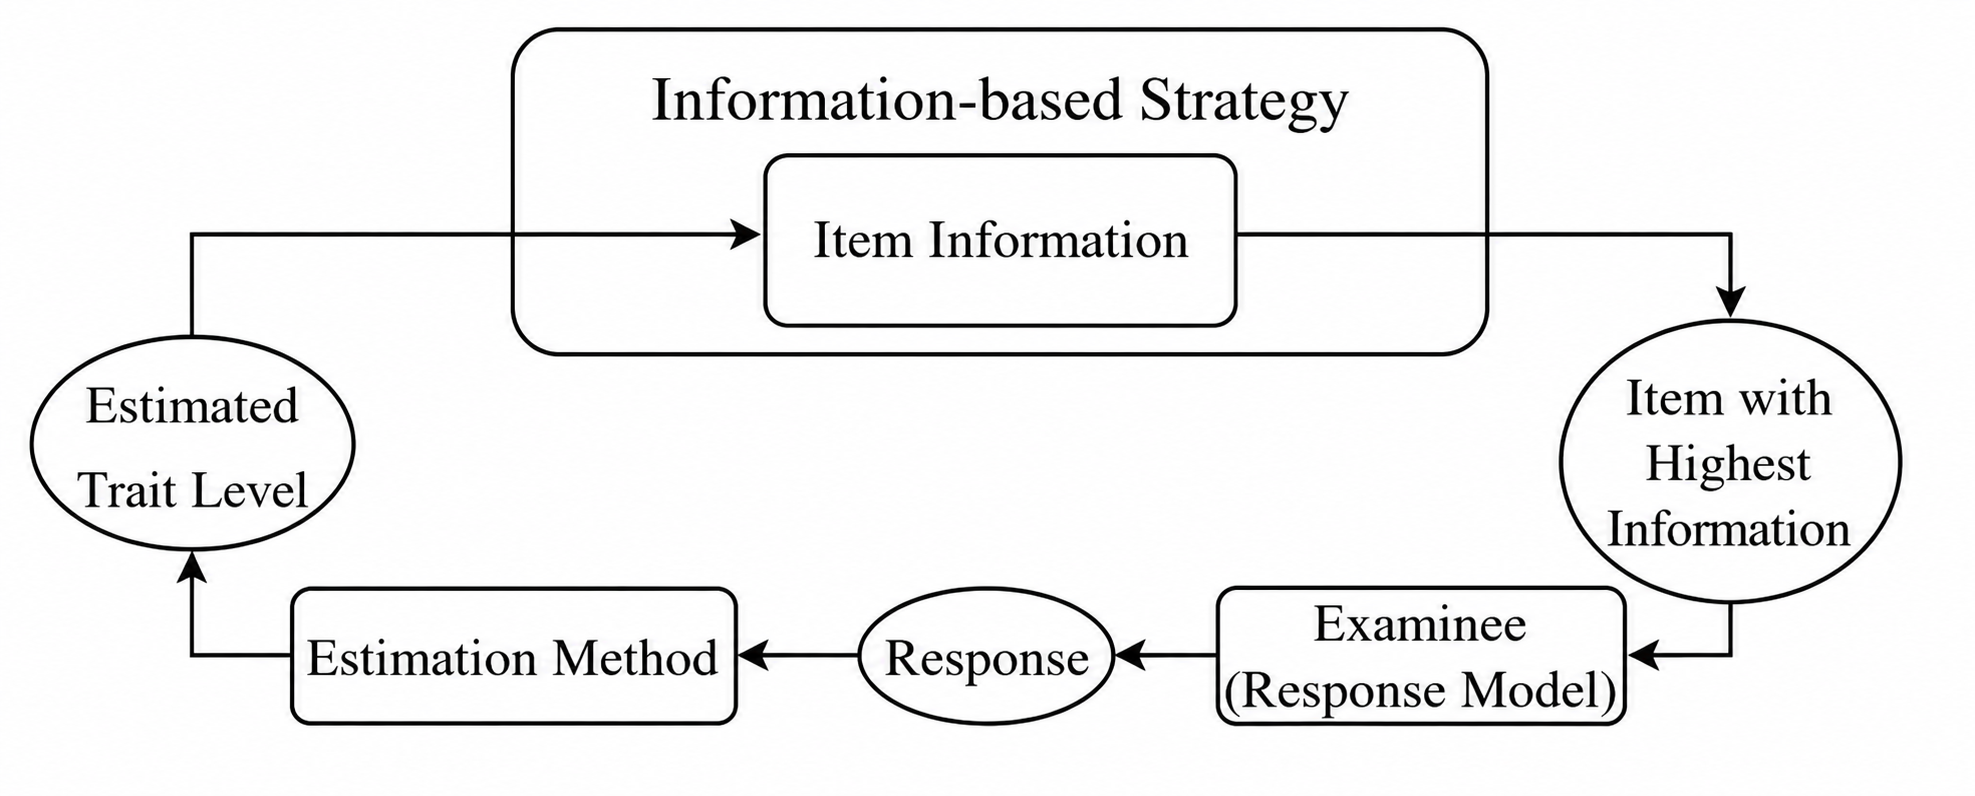
\includegraphics[width=.92\columnwidth]{img/irt_flow.png}
\caption{IRT ベースの項目選択戦略のフローチャート．情報量基準に基づく戦略では，推定特性値から項目情報量を計算し，最も情報量の高い項目を選択する．}
\label{fig:irt_flow}
\end{figure}

\subsection{MDP に基づく定式化（DQN）}

Wang ら~\cite{wang2024} は，CAT の項目選択問題を MDP として定式化した．その構成要素は以下の通りである．
\begin{itemize}
\item 状態：現在の推定特性値 $\hat{\theta}_l$
\item 行動：選択する項目 $i_l \in B_l$
\item 報酬：項目 $i_l$ のフィッシャー情報量 $I_{i_l}(\theta)$\footnote{Wang らは報酬を推定特性値 $\hat{\theta}_l$ で計算しているが，本研究のシミュレーション実験では真の特性値 $\theta$ が既知であるため，より安定した報酬信号として真の $\theta$ を用いた．}
\item 環境：受検者の回答生成（IRT モデル）と特性値の推定（MLE）
\end{itemize}

\begin{figure}[t]
\centering
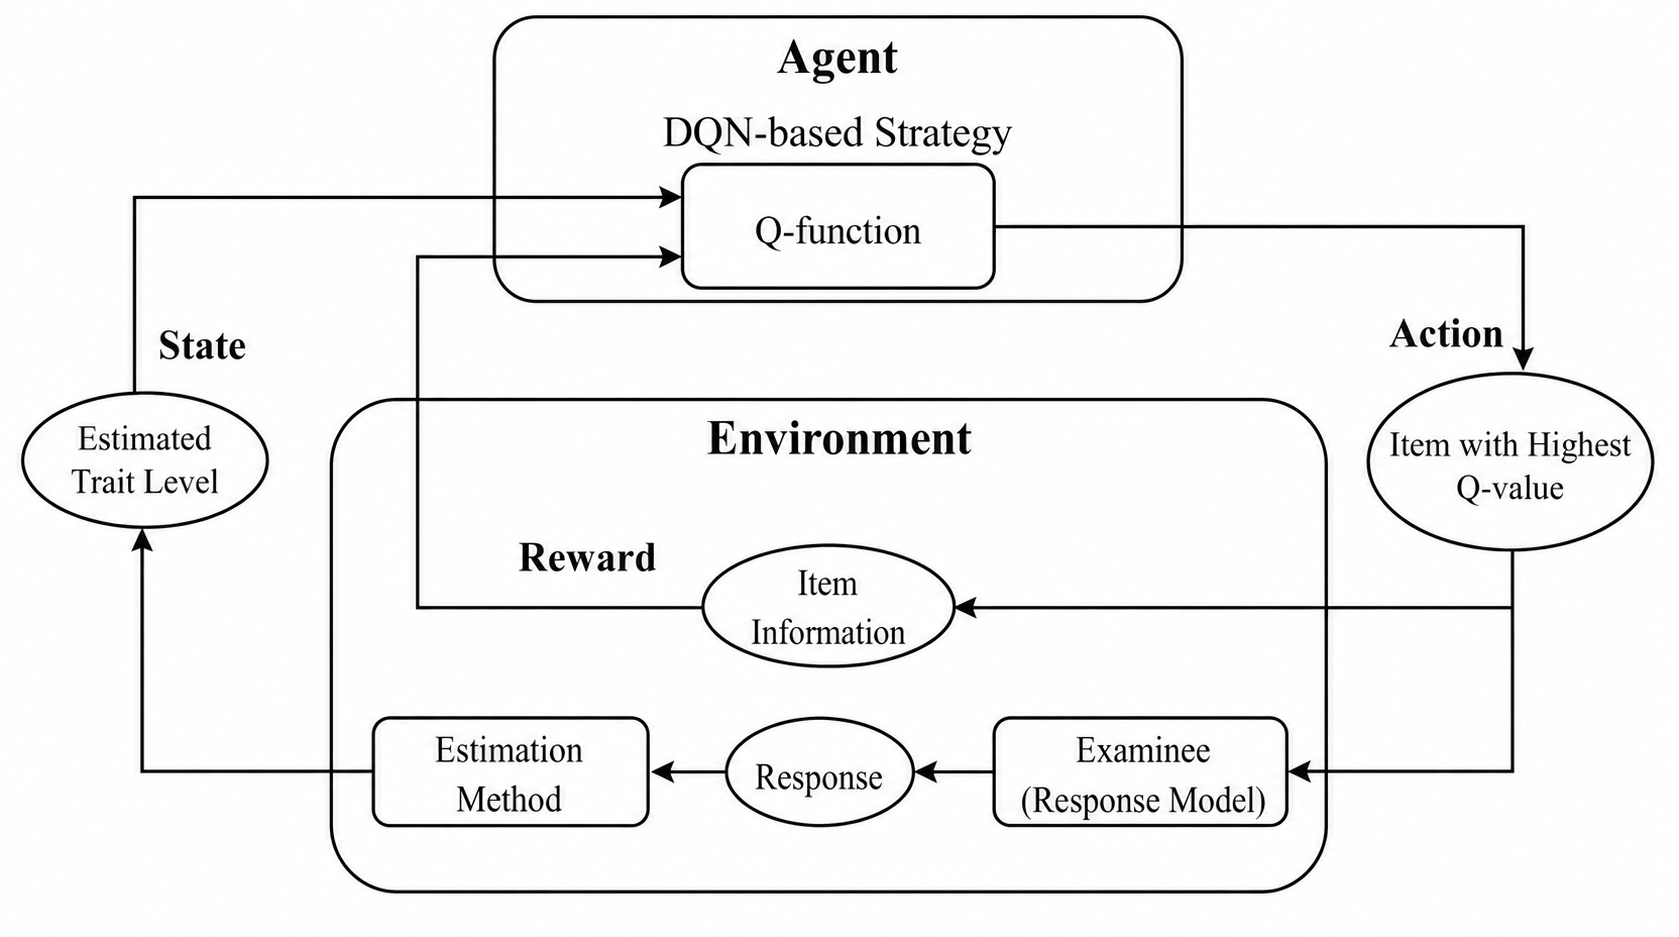
\includegraphics[width=.94\columnwidth]{img/mdp_flow.png}
\caption{MDP 枠組みにおける RL ベースの項目選択戦略のフローチャート．項目選択の基準が情報量の直接最大化から Q 値の最大化に置き換わり，将来のテスト全体を通じた累積報酬を考慮できる．}
\label{fig:mdp_flow}
\end{figure}

Q 関数は，現在の状態と行動の組に対して，テスト終了までに得られる割引累積報酬の期待値を表す．
\begin{equation}
Q^\pi(\hat{\theta}_l, i_l)
= \mathbb{E}_\pi \left[
I_{i_l}(\hat{\theta}_l)
+ \sum_{k=l+1}^{L} \gamma^{k-l} I_{i_k}(\hat{\theta}_k)
\mid \hat{\theta}_l, i_l
\right]
\end{equation}
ここで $\gamma$ は割引率，$L$ はテスト長である．DQN は Q-Network $Q(\hat{\theta}_l, i; \bm{\theta})$ を用いてこの Q 関数を近似する．

\begin{figure}[t]
\centering
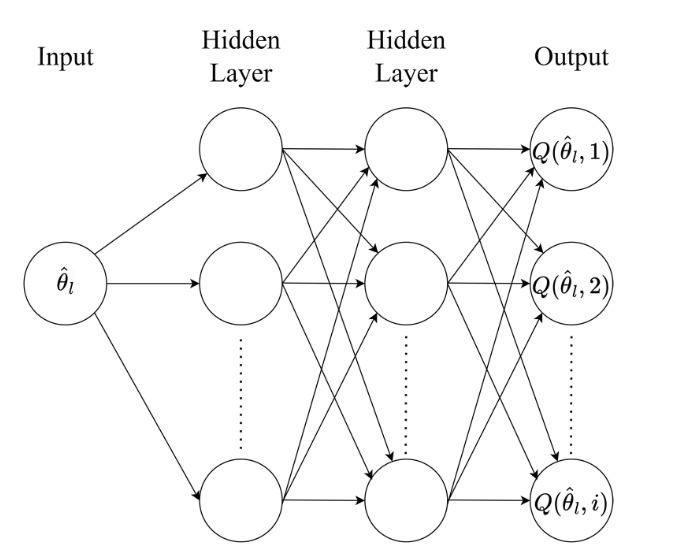
\includegraphics[width=.88\columnwidth]{img/dqn_arch.png}
\caption{DQN における Q-Network のアーキテクチャ．入力は推定特性値 $\hat{\theta}_l$ であり，2層の全結合ネットワークを経て各項目の Q 値を出力する．}
\label{fig:dqn_arch}
\end{figure}

\section{提案手法}

\subsection{POMDP としての再定式化}

Wang らの MDP 定式化では，状態を推定特性値 $\hat{\theta}_l$ とする．しかし，推定特性値は真の特性値 $\theta$ の不完全な推定であり，特にテスト序盤では大きな誤差を含む．つまり，エージェントは真の状態を直接観測できず，観測される回答の正誤を通じて間接的に推論するしかない．これは部分観測マルコフ決定過程（POMDP）の構造そのものである．

そこで本研究では，CAT の項目選択問題を次のような POMDP として再定式化する．
\begin{itemize}
\item 真の状態：受検者の真の特性値 $\theta$
\item 観測：各項目への回答 $o_l \in \{0,1\}$
\item 行動：選択する項目 $i_l \in B_l$
\item 報酬：フィッシャー情報量 $I_{i_l}(\theta)$
\end{itemize}
POMDP において，エージェントは観測履歴 $h_l=(o_1,\ldots,o_{l-1})$ から真の状態に関する信念を構築し，行動を選択する．

\subsection{DRQN による Q 関数の近似}

POMDP を解くため，Hausknecht と Stone~\cite{hausknecht2015} が提案した DRQN を用いる．DRQN は DQN の全結合層を LSTM に置き換えたアーキテクチャであり，過去の観測系列を逐次処理することで，部分観測下での Q 値推定を可能にする．

本研究における DRQN のアーキテクチャは以下の構成である．
\begin{enumerate}
\item Embedding 層：回答を3カテゴリ（0: 誤答，1: 正答，2: 開始トークン）の埋め込み表現に変換する．
\item LSTM 層：埋め込み系列を逐次処理し，隠れ状態を更新する．
\item 全結合出力層：LSTM の出力からアイテムバンク内の全項目に対する Q 値を出力する．
\end{enumerate}

\begin{figure}[t]
\centering
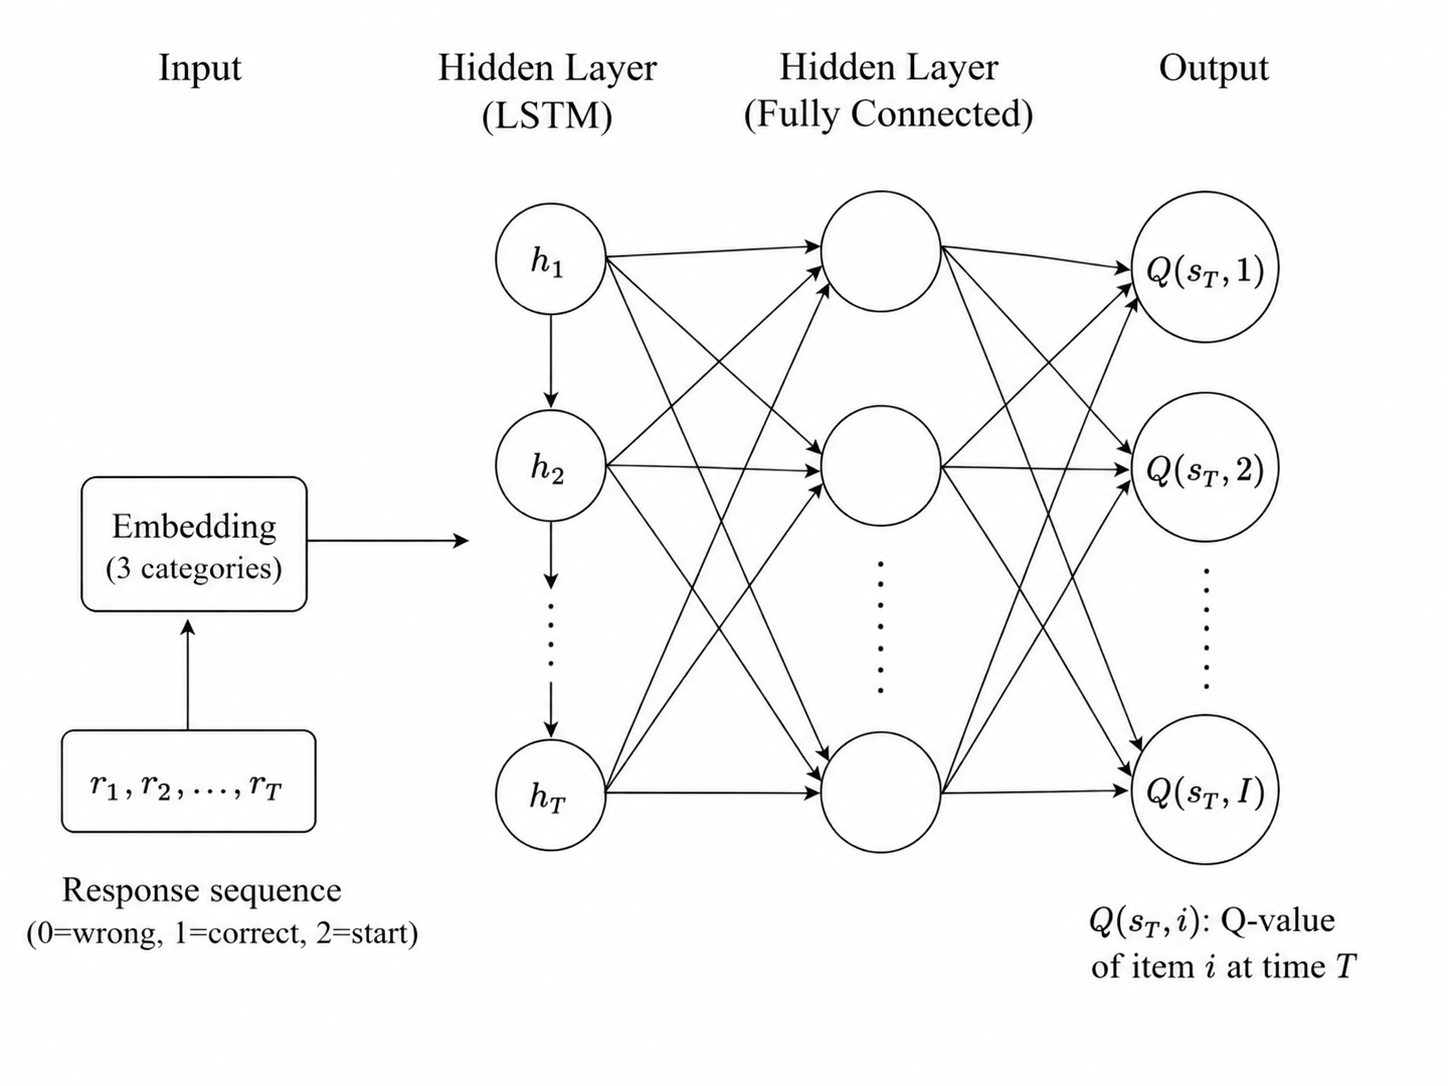
\includegraphics[width=.88\columnwidth]{img/drqn_arch.png}
\caption{DRQN のアーキテクチャ．回答系列を Embedding 層で埋め込み表現に変換し，LSTM で逐次処理した後，各項目の Q 値を出力する．}
\label{fig:drqn_arch}
\end{figure}

決定ステップ $l$ において，DRQN は開始トークンとこれまでの回答系列 $(\text{START}, o_1, o_2, \ldots, o_{l-1})$ を入力として受け取り，LSTM が内部状態を逐次更新する．これにより，推定特性値というスカラー情報に集約せずに，回答パターンの時系列的な特徴を直接利用して Q 値を推定する．

\begin{table}[t]
\centering
\caption{DQN と DRQN の比較}
\label{tab:dqn_drqn}
\scriptsize
\setlength{\tabcolsep}{3pt}
\begin{tabular}{p{0.18\columnwidth}p{0.30\columnwidth}p{0.34\columnwidth}}
\toprule
 & DQN & DRQN \\
\midrule
定式化 & MDP & POMDP \\
状態表現 & 推定特性値 $\hat{\theta}_l$ & 回答履歴 $(o_1,\ldots,o_{l-1})$ \\
ネットワーク & 全結合ネットワーク & Embedding + LSTM + 全結合 \\
入力次元 & 1 & 可変長系列 \\
\bottomrule
\end{tabular}
\end{table}

\subsection{学習アルゴリズム}

DRQN の学習は DQN と同様に，$\varepsilon$-greedy 法による方策選択，ターゲットネットワーク，および経験再生（experience replay）の3つの手法を用いる~\cite{mnih2013,mnih2015}．

ただし，Wang らの DQN では経験再生の単位がステップごとの遷移 $\{\hat{\theta}_l, i_l, I_{i_l}(\hat{\theta}_l), \hat{\theta}_{l+1}\}$ であるのに対し，本研究の DRQN では経験再生の単位を1エピソード（1人の受検者のテスト全体）とする．これは，LSTM の隠れ状態がエピソード内の回答系列に依存しており，系列の途中の単一遷移だけを抜き出すと隠れ状態を正しく再現できないためである．

学習の手順は以下の通りである．
\begin{enumerate}
\item 学習用の特性値 $\theta_n$（$n = 1,\ldots,N_{\mathrm{training}}$）を生成する．
\item 各受検者について，テスト長 $L$ の CAT を実行し，各ステップの回答，行動，報酬を記録する．
\item エピソード単位でリプレイメモリに保存する．
\item ミニバッチをサンプリングし，次の損失関数で Q-Network のパラメータを更新する．
\end{enumerate}
\begin{align}
\mathcal{L}
= \Bigl[
r_l + \gamma \max_{i \in B_{l+1}} Q_{\mathrm{target}}(s_{l+1}, i; \bm{\theta}') \notag\\
&\qquad - Q_{\mathrm{action}}(s_l, i_l; \bm{\theta})
\Bigr]^2
\end{align}
さらに，$\tau$ 回の更新ごとにターゲットネットワークのパラメータを同期し，定期的にバリデーションを行って最良モデルを保存する．

\begin{figure}[t]
\centering
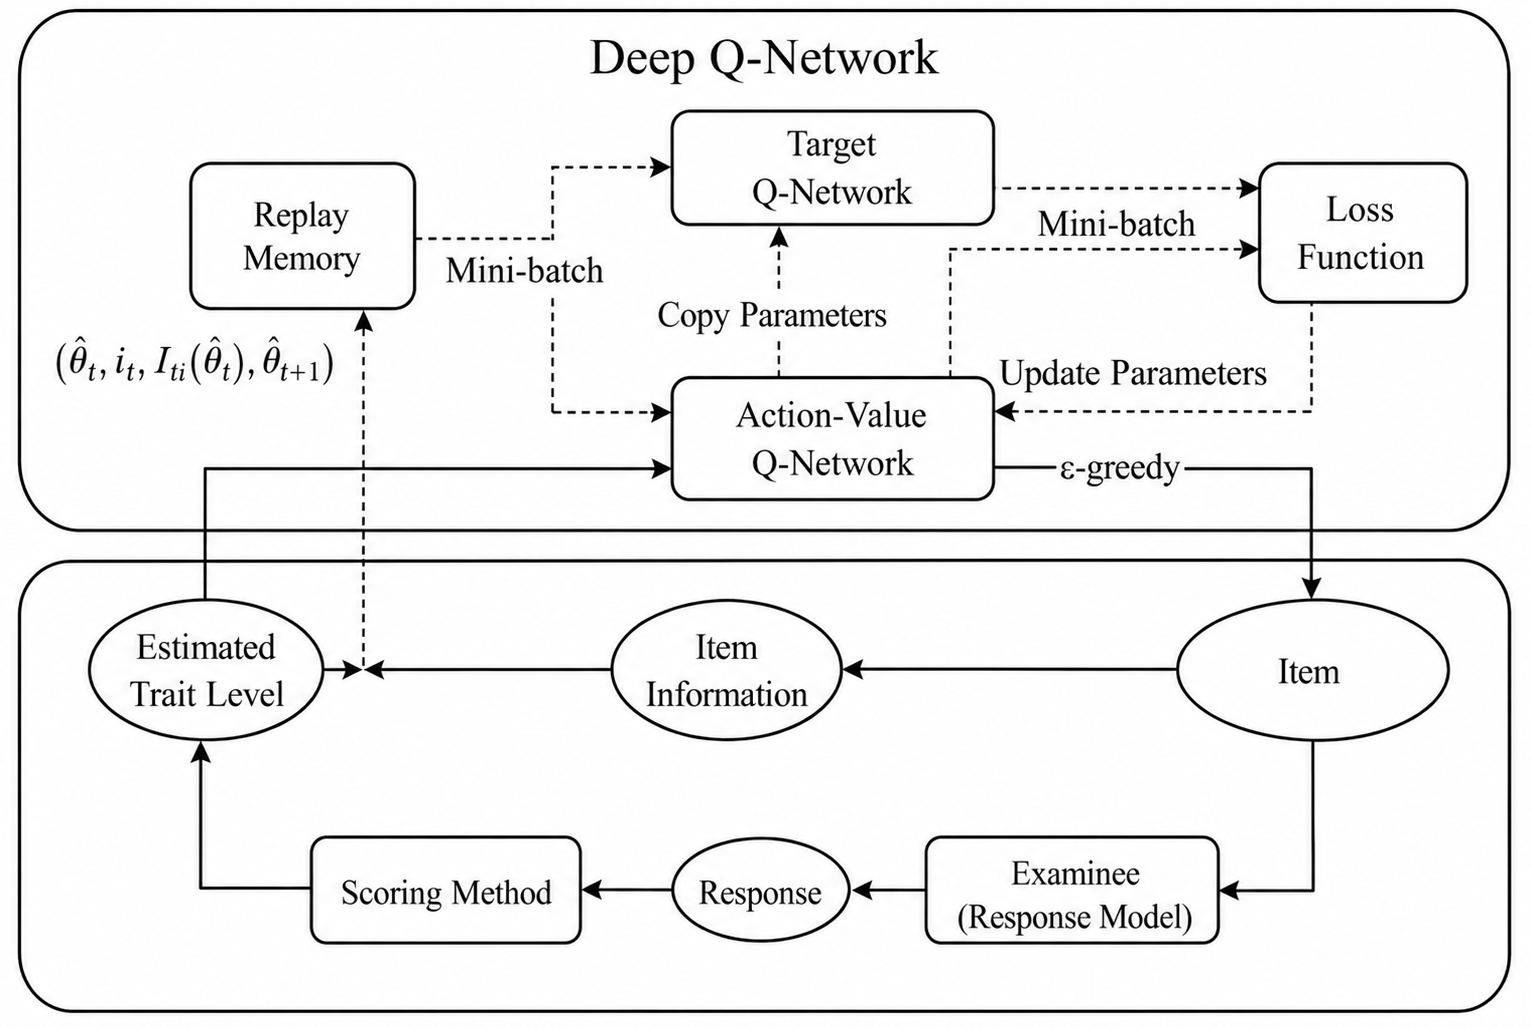
\includegraphics[width=.94\columnwidth]{img/dqn_training_flow.png}
\caption{DQN ベースの項目選択戦略の学習過程．DRQN では状態表現が回答履歴に置き換わり，経験再生の単位がステップからエピソードへ変更される．}
\label{fig:dqn_training}
\end{figure}

\section{シミュレーション実験}

\subsection{実験設定}

\paragraph{アイテムバンクの生成}
Wang ら~\cite{wang2024} のシミュレーション設定に基づき，各アイテムバンクを200項目で生成した．項目パラメータの分布は以下の通りである．
\begin{itemize}
\item 識別力：$a \sim N(1.2, 0.25)$（$a > 0$）
\item 困難度：$b \sim N(0, 1)$
\item 疑似推測：$c \sim N(0.25, 0.02)$（$0 < c < 1$）
\end{itemize}
パラメータ間に相関のないアイテムバンク（$r_{ab}=0$）と相関のあるアイテムバンク（$r_{ab}=0.5$）の2種類を各10バンク，計20バンク生成した．各バンクに対して，5,000名の受検者の真の特性値を標準正規分布 $N(0,1)$ から生成した．

\paragraph{比較手法}
以下の4手法を比較する．
\begin{enumerate}
\item MFI：最大フィッシャー情報量法~\cite{lord1980}
\item FIWL：尤度重み付きフィッシャー情報量法~\cite{veerkamp1997}
\item DQN：Deep Q-Network に基づく手法~\cite{wang2024}
\item DRQN：Deep Recurrent Q-Network に基づく手法（提案手法）
\end{enumerate}
MFI と FIWL の実装には R パッケージ catR~\cite{magis2017} を用いる．

\paragraph{強化学習手法のハイパーパラメータ}
DQN と DRQN の学習設定を表~\ref{tab:hyperparams} に示す．

\begin{table}[t]
\centering
\caption{DQN と DRQN のハイパーパラメータ}
\label{tab:hyperparams}
\scriptsize
\setlength{\tabcolsep}{3pt}
\begin{tabular}{p{0.28\columnwidth}p{0.22\columnwidth}p{0.33\columnwidth}}
\toprule
パラメータ & DQN & DRQN \\
\midrule
ネットワーク構造 & \shortstack[l]{1$\to$50\\$\to$30$\to$200} & \shortstack[l]{Embedding(3,16)\\$\to$LSTM(64)\\$\to$Linear(200)} \\
学習データ数 $N_{\mathrm{training}}$ & 1,000 & 1,000 \\
テスト長 $L$ & 40 & 40 \\
割引率 $\gamma$ & 0.1 & 0.1 \\
リプレイメモリサイズ $N_D$ & 1,000 & 1,000 \\
ミニバッチサイズ $m$ & 128 & 128 \\
ターゲット更新間隔 $\tau$ & 40 & 40 \\
学習率 & 0.001 & 0.001 \\
$\varepsilon$ & 0.1 & 0.1 \\
バリデーション間隔 & 50 & 50 \\
バリデーション数 & 200 & 200 \\
学習データ分布 & $N(0,1)$ & $N(0,1)$ \\
報酬 & $I_{i_l}(\theta)$ & $I_{i_l}(\theta)$ \\
\bottomrule
\end{tabular}
\end{table}

DQN では全てのネットワークパラメータに正値制約を適用し，Q 値が正であることを保証する．DRQN では出力層の重みとバイアスのみに正値制約を適用し，さらに勾配クリッピング（最大ノルム 1.0）を導入して学習を安定化させる．

\paragraph{評価指標}
以下の3指標を用いて，推定特性値の回復精度を評価する．
\begin{equation}
\mathrm{Bias} = \frac{1}{N} \sum_{n=1}^{N} (\hat{\theta}_n - \theta_n)
\end{equation}
\begin{equation}
\mathrm{RMSE} = \sqrt{\frac{1}{N} \sum_{n=1}^{N} (\hat{\theta}_n - \theta_n)^2}
\end{equation}
\begin{equation}
\mathrm{MAE} = \frac{1}{N} \sum_{n=1}^{N} \lvert \hat{\theta}_n - \theta_n \rvert
\end{equation}

\subsection{結果}

無相関アイテムバンク（$r_{ab}=0$，バンク1）におけるテスト長40時点での比較結果を表~\ref{tab:step40_results} に示す．

\begin{table}[t]
\centering
\caption{無相関バンク（バンク1）における40問選択時点の推定精度}
\label{tab:step40_results}
\small
\begin{tabular}{lccc}
\toprule
手法 & Bias & RMSE & MAE \\
\midrule
MFI & 0.012 & 0.342 & 0.264 \\
FIWL & --- & --- & --- \\
DQN ($\gamma=0.1$, normal) & -0.028 & 0.254 & 0.170 \\
DRQN ($\gamma=0.1$, normal) & -0.101 & 0.200 & 0.157 \\
\bottomrule
\end{tabular}
\end{table}

DRQN は40問選択時点において RMSE = 0.200 を達成し，MFI（RMSE = 0.342）と比較して約42\%，DQN（RMSE = 0.254）と比較して約21\%の改善を示した．MAE についても同様の傾向が確認された．

各ステップにおける RMSE の推移を表~\ref{tab:rmse_by_step} に示す．

\begin{table}[t]
\centering
\caption{各ステップにおける RMSE の推移（無相関バンク，バンク1）}
\label{tab:rmse_by_step}
\small
\begin{tabular}{cccc}
\toprule
ステップ & MFI & DQN & DRQN \\
\midrule
5  & 0.984 & 0.852 & 1.078 \\
10 & 0.699 & 0.519 & 0.829 \\
15 & 0.547 & 0.424 & 0.544 \\
20 & 0.470 & 0.239 & 0.653 \\
25 & 0.418 & 0.260 & 0.366 \\
30 & 0.383 & 0.369 & 0.333 \\
35 & 0.358 & 0.294 & 0.191 \\
40 & 0.342 & 0.254 & 0.200 \\
\bottomrule
\end{tabular}
\end{table}

表~\ref{tab:rmse_by_step} に示すように，MFI は初期ステップから安定して RMSE が低下する．DQN もテスト序盤から比較的低い RMSE を示す．一方，DRQN はテスト序盤では MFI より高い RMSE を示すが，ステップ数が増加するにつれて急速に改善し，ステップ25以降では他の手法を上回る精度を達成する．これは，十分な回答履歴が蓄積されることで，LSTM が回答パターンから特性値の情報をより正確に抽出できるようになるためと考えられる．

\section{おわりに}

本研究では，IRT に基づく CAT の項目選択問題を POMDP として再定式化し，回答履歴を状態として利用する DRQN に基づく項目選択戦略を提案した．シミュレーション実験により，提案手法は40問選択時点において既存の MFI および DQN を上回る推定精度を達成することが示された．

提案手法の利点として，回答パターンの直接利用と，CAT を部分観測問題として扱う理論的整合性が挙げられる．一方で，テスト序盤の精度，バンク間の一般化，実データによる検証は今後の課題である．特に序盤性能の補完には，MFI 等の情報量基準手法を併用するハイブリッド戦略の検討が有望である．

\begin{thebibliography}{99}

\bibitem{barnhart2007}
H.~X. Barnhart, M.~J. Haber, and L.~I. Lin:
Overall concordance correlation coefficient for evaluating agreement among multiple observers,
\textit{Biometrics}, Vol.~63, No.~4, pp.~1099--1106 (2007)

\bibitem{chang1996}
H.-H. Chang and Z. Ying:
A global information approach to computerized adaptive testing,
\textit{Applied Psychological Measurement}, Vol.~20, No.~3, pp.~213--229 (1996)

\bibitem{chen2018}
Y. Chen, X. Li, J. Liu, and Z. Ying:
Recommendation system for adaptive learning,
\textit{Applied Psychological Measurement}, Vol.~42, No.~1, pp.~24--41 (2018)

\bibitem{dodd1990}
B.~G. Dodd:
The effect of item selection procedure and stepsize on computerized adaptive attitude measurement using the rating scale model,
\textit{Applied Psychological Measurement}, Vol.~14, No.~4, pp.~355--366 (1990)

\bibitem{frey2023}
A. Frey:
Computerized adaptive testing,
in R.~J. Mislevy and H. Jiao (Eds.),
\textit{The Oxford Handbook of Educational Assessment},
Oxford University Press (2023)

\bibitem{ghosh2021}
A. Ghosh and A. Lan:
BOBCAT: Bilevel optimization-based computerized adaptive testing,
\textit{arXiv preprint arXiv:2108.07386} (2021)

\bibitem{han2020}
R. Han, K. Chen, and C. Tan:
Curiosity-driven recommendation strategy for adaptive learning via deep reinforcement learning,
\textit{British Journal of Mathematical and Statistical Psychology},
Vol.~73, No.~3, pp.~522--540 (2020)

\bibitem{hausknecht2015}
M. Hausknecht and P. Stone:
Deep recurrent Q-learning for partially observable MDPs,
\textit{arXiv preprint arXiv:1507.06527} (2015)

\bibitem{li2021}
X. Li, H. Xu, J. Zhang, and H.-H. Chang:
Optimal hierarchical learning path design with reinforcement learning,
\textit{Applied Psychological Measurement}, Vol.~45, No.~1, pp.~54--70 (2021)

\bibitem{li2023}
X. Li, H. Xu, J. Zhang, and H.-H. Chang:
Deep reinforcement learning for adaptive learning systems,
\textit{Journal of Educational and Behavioral Statistics},
Vol.~48, No.~2, pp.~220--243 (2023)

\bibitem{lord1980}
F.~M. Lord:
\textit{Applications of Item Response Theory to Practical Testing Problems},
Erlbaum (1980)

\bibitem{magis2017}
D. Magis and J.~R. Barrada:
Computerized adaptive testing with R: Recent updates of the package catR,
\textit{Journal of Statistical Software}, Vol.~76, No.~1, pp.~1--19 (2017)

\bibitem{mnih2013}
V. Mnih, K. Kavukcuoglu, D. Silver, \textit{et al}.:
Playing Atari with deep reinforcement learning,
\textit{arXiv preprint arXiv:1312.5602} (2013)

\bibitem{mnih2015}
V. Mnih, K. Kavukcuoglu, D. Silver, \textit{et al}.:
Human-level control through deep reinforcement learning,
\textit{Nature}, Vol.~518, No.~7540, pp.~529--533 (2015)

\bibitem{nurakhmetov2019}
D. Nurakhmetov:
Reinforcement learning applied to adaptive classification testing,
in B.~P. Veldkamp and C. Sluijter (Eds.),
\textit{Theoretical and Practical Advances in Computer-based Educational Measurement},
pp.~325--336, Springer (2019)

\bibitem{shin2022}
J. Shin and O. Bulut:
Building an intelligent recommendation system for personalized test scheduling in computerized assessments: A reinforcement learning approach,
\textit{Behavior Research Methods}, Vol.~54, No.~1, pp.~216--232 (2022)

\bibitem{silver2016}
D. Silver, A. Huang, C.~J. Maddison, \textit{et al}.:
Mastering the game of Go with deep neural networks and tree search,
\textit{Nature}, Vol.~529, No.~7587, pp.~484--489 (2016)

\bibitem{silver2017}
D. Silver, J. Schrittwieser, K. Simonyan, \textit{et al}.:
Mastering the game of Go without human knowledge,
\textit{Nature}, Vol.~550, No.~7676, pp.~354--359 (2017)

\bibitem{sutton2018}
R.~S. Sutton and A.~G. Barto:
\textit{Reinforcement Learning: An Introduction},
2nd ed., MIT Press (2018)

\bibitem{tan2020}
C. Tan, R. Han, R. Ye, and K. Chen:
Adaptive learning recommendation strategy based on deep Q-learning,
\textit{Applied Psychological Measurement}, Vol.~44, No.~4, pp.~251--266 (2020)

\bibitem{tang2019}
X. Tang, Y. Chen, X. Li, J. Liu, and Z. Ying:
A reinforcement learning approach to personalized learning recommendation systems,
\textit{British Journal of Mathematical and Statistical Psychology},
Vol.~72, No.~1, pp.~108--135 (2019)

\bibitem{vanderlinden2016}
W.~J. van der Linden:
\textit{Handbook of Item Response Theory},
CRC Press (2016)

\bibitem{veerkamp1997}
W.~J.~J. Veerkamp and M.~P.~F. Berger:
Some new item selection criteria for adaptive testing,
\textit{Journal of Educational and Behavioral Statistics},
Vol.~22, No.~2, pp.~203--226 (1997)

\bibitem{wainer2000}
H. Wainer, N.~J. Dorans, D. Eignor, \textit{et al}.:
\textit{Computerized Adaptive Testing: A Primer},
2nd ed., Erlbaum (2000)

\bibitem{wang2024}
P. Wang, H. Liu, and M. Xu:
An adaptive testing item selection strategy via a deep reinforcement learning approach,
\textit{Behavior Research Methods}, Vol.~56, pp.~8695--8714 (2024)

\bibitem{weiss1982}
D.~J. Weiss:
Improving measurement quality and efficiency with adaptive testing,
\textit{Applied Psychological Measurement}, Vol.~6, No.~4, pp.~473--492 (1982)

\bibitem{weiss1984}
D.~J. Weiss and G.~G. Kingsbury:
Application of computerized adaptive testing to educational problems,
\textit{Journal of Educational Measurement}, Vol.~21, No.~4, pp.~361--375 (1984)

\bibitem{zhang2016}
J. Zhang and H.-H. Chang:
From smart testing to smart learning: How testing technology can assist the new generation of education,
\textit{International Journal of Smart Technology and Learning},
Vol.~1, No.~1, pp.~67--92 (2016)

\end{thebibliography}

\end{document}
